\documentclass[a4paper]{article} 
\usepackage[a4paper,  fancysections,  titlepage]{polytechnique}
\usepackage[backend=biber, style=numeric]{biblatex}
\usepackage[english]{babel}
\usepackage[T1]{fontenc}
\usepackage{blindtext}
\usepackage[hidelinks]{hyperref}
\usepackage{amsmath, amssymb}
\usepackage{parskip}
\usepackage{graphicx}
\usepackage{wrapfig}
\usepackage{bm}
\usepackage{braket}
\usepackage{csquotes}
\usepackage{caption}
\usepackage{cleveref}
\usepackage{subcaption}

\graphicspath{{../figures/}}

\addbibresource{refs.bib}

\titleformat{\subsection}
  [block]
  {\color{bleu315}\sffamily\mdseries\large}
  {\thesubsection}
  {0.3em}
  {}  

\newcommand{\code}[1]{%
    \mbox{\ttfamily%
        \detokenize{#1}%
    }%
}

\newcommand{\resultat}[1]{%
    \quad \rightsquigarrow \quad #1%
}
\setlength{\parindent}{0pt}

\newcommand{\Worldline}[0]{\code{Worldline}}

\title{World-Line Quantum Monte Carlo}
\author{Victor Caro \& Théa Araujo}
\date{December 2025}

\begin{document}

\maketitle

\begin{abstract}
    The objective of this project is to implement the algorithm proposed by \textcite{Assaad2008}: a world-line approach to quantum Monte Carlo methods for one-dimensional XXZ Heisenberg spin chains.
\end{abstract}

\tableofcontents

\section{Introduction}

Problems in solid-state physics often require computationally demanding calculations, as their complexity typically scales as a power of system size. Spin chains and electron chains exhibit strong correlations, making exact solutions infeasible for large systems. However, one-dimensional (1D) spin chains provide a good balance between analytical tractability and physical relevance. In this study, the focus is placed on 1D XXZ chains, where correlations along the $x$ and $y$ axes are identical. This framework allows verification of theoretical predictions, assessment of approximations, and extrapolation of system properties to larger sizes. The Monte Carlo method described in \cite{Assaad2008} was implemented using three distinct update schemes.

\subsection{The XXZ Hamiltonian}

The XXZ model describes a chain of interacting spin-$\frac{1}{2}$ particles with nearest-neighbour coupling and anisotropy between the $xy$-plane and the $z$-direction. The Hamiltonian is given by

\begin{equation}
    H = J_{x}\sum_{i}(S_{i}^{x}S_{i+1}^{x} + S_{i}^{y}S_{i+1}^{y}) + J_{z}\sum_{i}S_{i}^{z}S_{i+1}^{z}
\end{equation}

Periodic boundary conditions are imposed such that $S_i = S_{i+n}$. The coupling constants $J_x$ and $J_z$ define the physical regime of the system: the $J_z$ term represents an Ising-like interaction, favouring spin alignment ($J_z<0$) or anti-alignment ($J_z>0$), whereas $J_x$ induces quantum fluctuations through spin exchanges between neighbouring sites.

\subsection{Computational complexity}

Although the Hamiltonian can be written compactly, evaluating thermodynamic quantities such as specific heat, magnetic susceptibility, or spin stiffness requires computation of the partition function $Z = \mathrm{Tr}[e^{-\beta H}]$.

This presents a mathematical challenge: the Hilbert space of a quantum system grows exponentially with its physical size. Since each local spin has two basis states ($\ket{\uparrow}$ and $\ket{\downarrow}$), the dimension of the total Hilbert space is:

\begin{equation}
    \text{dim}(\mathcal{H}_n) = 2^n
\end{equation}

For very small systems, one can perform diagonalization of the Hamiltonian matrix. However, this approach becomes impossible for large systems. Therefore, it is necessary to use other numerical approaches to solve for larger systems that do not require the full matrix diagonalization. Nevertheless, this exact calculation is crucial for testing the numerical method on smaller systems and for extrapolating to larger ones.


\section{World-line approach}

\subsection{Trotterization}

Following the derivation by \textcite{Assaad2008}, the problem is simplified to make it tractable numerically. Let $H^{(i)} = J_{x}(S_{i}^{x}S_{i+1}^{x} + S_{i}^{y}S_{i+1}^{y}) + J_{z}S_{i}^{z}S_{i+1}^{z}$ be the two-site Hamiltonian, whose eigenvalues are known. Then, $H_1$, the sum of the even two-sites, and $H_2$, the sum of the odd terms, are two sums of commuting Hamiltonians. Introducing the discretisation $\Delta\tau \equiv \frac{\beta}{m}$, Trotter’s formula approximates the partition function as:

\begin{align*}
    Z &= \text{Tr}[(e^{-\Delta\tau H})^{m}] \\
        &= \text{Tr}[(e^{-\Delta\tau  H_{1}}e^{-\Delta\tau  H_{2}})^{m}] + \mathcal{O}(\Delta\tau^{2}) \\
        &=\sum_{\pmb{\sigma}_1 \dots \pmb{\sigma}_{2m}} \bra{\pmb{\sigma}_1} e^{-\Delta\tau H_1} \ket{\pmb{\sigma}_{2m}} \cdots \braket{\pmb{\sigma}_2|e^{-\Delta\tau H_2}|\pmb{\sigma}_1} + \mathcal{O}(\Delta\tau^{2})
\end{align*}


Then, $\Delta\tau$ can then be interpreted as a discrete imaginary time step, mapping the 1D system into a 2D configuration with a progression from $\tau = 0$ to $\tau = m\Delta\tau = \beta$ as the additional dimension. This conversion allows to treat this system with a classical approach, thus enabling Monte Carlo methods.

\begin{figure}[!ht]
    \centering
    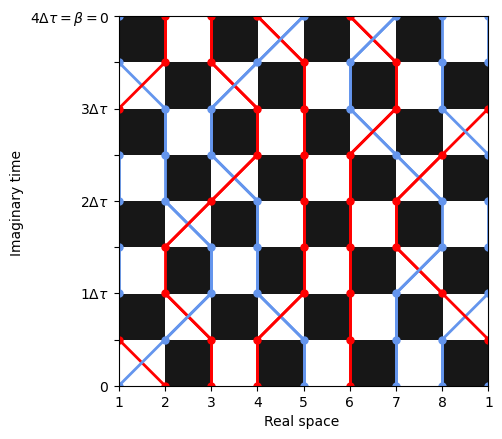
\includegraphics[width=0.8\textwidth]{World-lines 8x8.png}
    \caption{World-line configuration for $8$ spin sites and $m=4$. Red represents up spins and blue represents down spins.}
    \label{fig:8x8}
\end{figure}

This system can then be represented as a world-line configuration tracking the evolution of the chain's spin configurations through time and space. This representation possesses interesting properties, such as spin conservation, which simplifies the calculation by eliminating spin evolution or 2D configurations not having a meaningful contribution at first order on $\Delta\tau$.

Periodic boundary conditions are chosen as they ensure that boundary effects are minimised. In practice, $m$ needs to be large enough so as to minimise the effects of the Trotterization.

As for the code,a \Worldline{} is represented by a matrix of size $2m \times n$ containing $\pm1$ values depending on the state of the spin at that location.

\subsection{Weight and energy of world-lines}

Each \Worldline{} has its own weight denoted as $\Omega(\omega)$.

From \cite{Assaad2008}:

\begin{equation} \label{Omega_prod}
    \Omega(\omega) = \prod_{i=1}^{2m} \braket{\pmb{\sigma}_{i+1}|e^{-\Delta\tau H_i}|\pmb{\sigma}_{i}}
\end{equation}


Where $H_i$ is $H_1$ if $i$ is odd and $H_2$ otherwise. Periodic boundary conditions give $\pmb{\sigma}_{2m+1}=\pmb{\sigma}_{1}$.

With \cref{Omega_prod}, the total weight is the product of the weight of each line.

\begin{equation} \label{plaquette}
    \braket{\pmb{\sigma}_{i+1}|e^{-\Delta\tau H_i}|\pmb{\sigma}_i} =
    \prod_{j=i}^{n/2} \braket{\sigma_{2j, i+1}, \sigma_{2j+1, i+1} |e^{-\Delta\tau H_i}|\sigma_{2j,i},\sigma_{2j+1,i}}
\end{equation}

And \cref{plaquette} gives that each line weight is the product of the weight of each of its white plaquette.

\textit{Note: In the code} \code{i} \textit{and} \code{j} \textit{are switched from the usual convention to match the notation used in the paper.}

The combination of \cref{Omega_prod} and \cref{plaquette} gives a straightforward algorithm to compute the weight of a \Worldline:
\begin{equation}
     \Omega(\omega) = \prod_{p} W_p
\end{equation}
Where $p$ is taken over all white plaquettes of $\omega$ and $W_p$ is the plaquette weight.

The energy associated with a configuration is: (from \cite{Assaad2008})
\begin{equation}
    E(w) = -\frac{1}{m} \sum_{p} \frac{\partial}{\partial \Delta\tau} \ln(W_p)
\end{equation}

Based on the weights provided in \cite{Assaad2008} :

\begin{itemize}
    \item \textbf{Full Squares:}
    \begin{align}
        W &= e^{-\Delta\tau J_z / 4} \\
        -\frac{\partial}{\partial \Delta\tau} \ln(W) &= -\frac{\partial}{\partial \Delta\tau} \left( -\frac{\Delta\tau J_z}{4} \right) = \frac{J_z}{4}
    \end{align}

    \item \textbf{Vertical World-Lines:}
    \begin{align}
        W &= e^{\Delta\tau J_z / 4} \cosh\left(\frac{\Delta\tau J_x}{2}\right) \\
        -\frac{\partial}{\partial \Delta\tau} \ln(W) &= -\left( \frac{J_z}{4} + \frac{J_x}{2} \tanh\left(\frac{\Delta\tau J_x}{2}\right) \right)
    \end{align}

    \item \textbf{Crossed World-Lines:}
    \begin{align}
        W &= -e^{\Delta\tau J_z / 4} \sinh\left(\frac{\Delta\tau J_x}{2}\right) \\
        -\frac{\partial}{\partial \Delta\tau} \ln|W| &= -\left( \frac{J_z}{4} + \frac{J_x}{2} \coth\left(\frac{\Delta\tau J_x}{2}\right) \right)
    \end{align}
\end{itemize}

\subsection{Generating world-line configurations}

In order to test the validity of Trotter's formula and our calculation method, one can generate all possible valid configurations for small grids. This allows to make exact calculations and compare them to our results.

The first approach took was to generate all the spin configurations possible and to keep only the valid ones. While straightforward to implement, this approach was computationally inefficient, as it required computing $2^{2 m n}$ configurations.

The second approach consisted of recursively generating a world-line with backtracking whenever an invalid configuration was encountered. Enforcing periodic boundary conditions proved more difficult than expected, resulting in reduced implementation efficiency. Each world-line was generated until an invalid configuration appeared on a white plaquette, at which point the process was halted. However, this algorithm did not yield significant improvement over the previous one, as the number of configurations continued to grow exponentially. The method could be optimised by detecting invalid configurations earlier to avoid generating multiple invalid branches. Using this approach, all valid configurations were generated for systems with fewer than six sites and $m \le 4$ in under one minute. For eight sites at $m = 4$, computational limitations prevented full enumeration, although the number of valid configurations is estimated to exceed $10^6$.

\begin{table}[!ht]
\centering
\begin{tabular}{|c || c | c | c | c|} 
 \hline
 n/m & 1 & 2 & 3 & 4 \\ [0.5ex] 
 \hline \hline
  2 & 6 & 18 & 66 & 258 \\
  \hline
 4 & 18 & 90 & 546 & 3618 \\ [1ex] 
 \hline
  6 & 66 & 546 & 6840 & 94386 \\ [1ex] 
 \hline
  8 & 258 & 3618 & 94386 & - \\ [1ex] 
 \hline
\end{tabular}
\caption{Number of valid configurations for n sites and different values of m}
\label{table:2}
\end{table}

The generation of all world-lines enabled the computation of the Trotterization error which is shown in \cref{fig:energy_tau}.


\section{Metropolis algorithm}

To perform a complete Monte Carlo simulation, the Metropolis algorithm \cite{metropolis1949monte} was used and three different update schemes were implemented.

\subsection{Local shifts}

The first update approach is by shifting spin lines on a shaded plaquette. An illustration of this can be seen in \cref{local:combined}.

\begin{figure}[!ht]
    \centering
    
    \begin{subfigure}{0.3\textwidth}
        \centering
        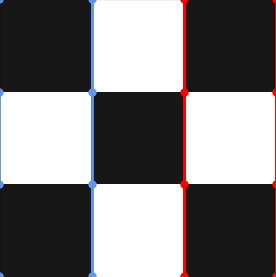
\includegraphics[width=\linewidth]{side.png}
        \caption{Configuration \textit{side}}
        \label{local:imageA}
    \end{subfigure}%
    \hfill%
    \begin{subfigure}{0.3\textwidth}
        \centering
        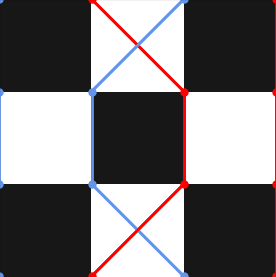
\includegraphics[width=\linewidth]{crossed.png}
        \caption{Configuration \textit{crossed}}
        \label{local:imageB}
    \end{subfigure}

    \caption{A local shift move}
    \label{local:combined}
\end{figure}

The advantage of this technique is its ease of implementation as the energy and weight shifts are trivial to compute, and the move has a symmetric probability.

The major drawback of this update method is that it is not ergodic. Indeed, the number of up spins remains the same throughout the move. This restricts the simulation to a subspace of the problem.

\subsection{Vertex update}

The second update method is inspired by \cite{Assaad2008} and uses the mapping to the 6-vertex problem.

\begin{figure}[!ht]
    \centering
    \begin{subfigure}[]{0.24\textwidth}
        \centering
        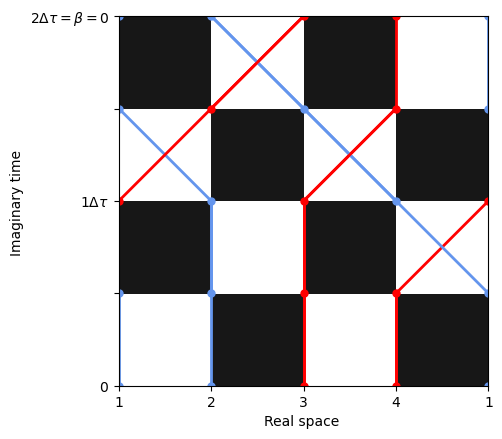
\includegraphics[width=\textwidth]{4x4 vertex 0.png}
        \caption{Initial configuration}
        \label{fig:graphe_a}
    \end{subfigure}
    \hfill 
    \begin{subfigure}[]{0.22\textwidth}
        \centering
        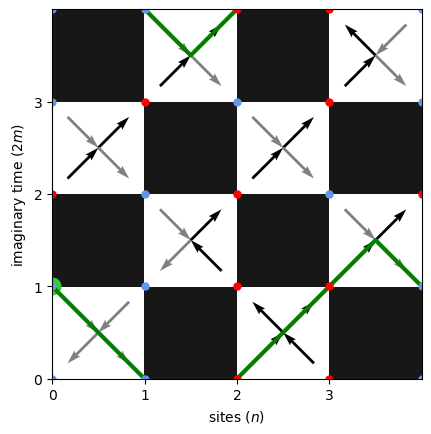
\includegraphics[width=\textwidth]{4x4 vertex 1.png}
        \caption{Vertex representation}
        \label{fig:graphe_b}
    \end{subfigure}
    \hfill
    \begin{subfigure}[]{0.22\textwidth}
        \centering
        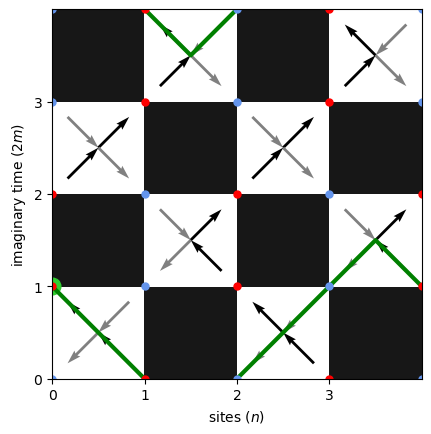
\includegraphics[width=\textwidth]{4x4 vertex 2.png}
        \caption{Loop transformation}
        \label{fig:graphe_c}
    \end{subfigure}
    \hfill
    \begin{subfigure}[]{0.24\textwidth}
        \centering
        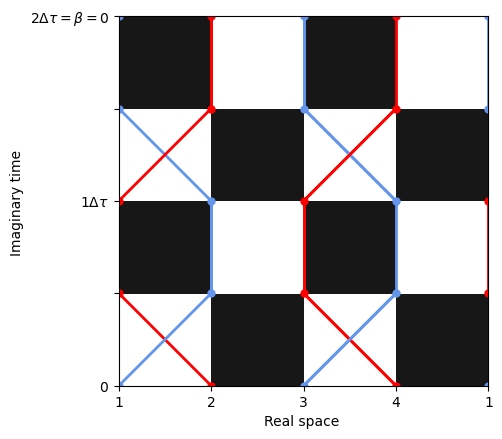
\includegraphics[width=\textwidth]{4x4 vertex 3.png}
        \caption{Final configuration}
        \label{fig:graphe_d}
    \end{subfigure}
    \hfill
    \caption{Metropolis algorithm with vertex update}
    \label{fig:comparaison_globale}
\end{figure}

Once the problem is mapped to the vertex representation, a random location is selected, and a random path is traced following the vertex orientations. This path necessarily returns to its starting point, forming a closed loop. The directions of the vertices encountered along the path are then inverted, producing another valid world-line configuration. Prior to the flip, the weight associated with the exchange along the loop is computed, as the move is subject to the Metropolis acceptance criterion. The transition probability is symmetric.

Any two configurations can be connected by flipping an appropriate set of loops, demonstrating ergodicity.

\textbf{The configurations differ by a finite number of loops.} -- Consider two configurations, $A$ and $B$, in their six-vertex representations. For each white plaquette, either $A$ and $B$ share the same vertex configuration or they contain two arrows in opposite directions. In the latter case, exactly two arrows must be reversed, since each square possesses two outgoing and two incoming arrows. Because the arrows form continuous loops across all world-lines, the set of differing arrows between $A$ and $B$ corresponds to a collection of closed loops.

\textbf{All loops are possible} -- Since paths are generated randomly and the visited plaquettes are chosen at random, any loop present in the configuration space can, in principle, be produced by the algorithm.

\subsection{Loop updates}

The last update method implemented is the one described in \cite{Assaad2008}.

It is first observed that each vertex configuration can be traversed in three distinct ways. Consequently, each plaquette is associated with three possible graphs, as illustrated in \cref{vertex_graph}.

\begin{figure}[!ht]
    \centering
    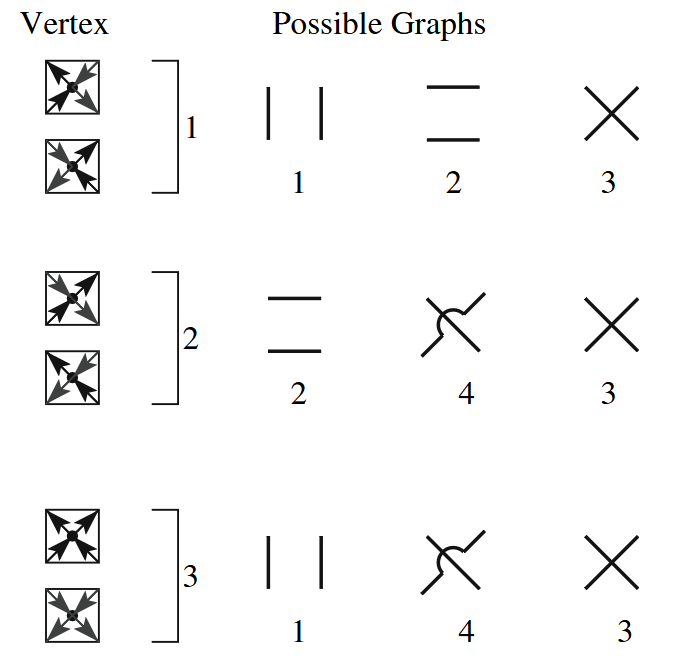
\includegraphics[width=0.5\textwidth]{loop_updates.png}
    \caption{Correspondence between vertex drawings and graphs. Taken from \textcite{Assaad2008} and adapted.}
    \label{vertex_graph}
\end{figure}

Weights are defined for each plaquette–graph combination as $W(S, G)$, where $S \in \{1, 2, 3\}$ denotes the plaquette type and $G \in \{1, 2, 3, 4\}$ denotes the graph, such that the normalisation condition holds.

\begin{equation} \label{sum_graph}
    W(S)=\sum_G W(S, G)
\end{equation}

From \cref{vertex_graph}, it follows that $W(1, 4) = W(2, 1) = W(3, 2) = 0$.

These weights are used to define the probability associated with selecting a particular graph.

\begin{equation}
    \mathbb{P}\left(S \to (S, G)\right) = \frac{W(S, G)}{W(S)}
\end{equation}

Once each plaquette has been mapped to a corresponding graph, multiple loops spanning the entire world-line configuration are obtained. A Union–Find data structure is employed to construct these loops, as illustrated in \cref{uf}.

\begin{figure}[!ht]
    \centering
    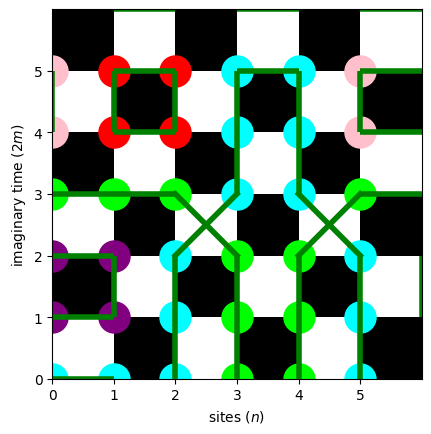
\includegraphics[width=0.5\textwidth]{uf.png}
    \caption{Partition of the word-line in loops. The green lines are the graphs. \textit{Note: the crossed lines represents graph 4 and not 3.}}
    \label{uf}
\end{figure}

For each loop defined by the graphs, it is then determined whether to flip the spins. The probability of such a flip is computed accordingly:
\begin{equation} \label{base_proba}
    \mathbb{P}\left((S, G) \to (S', G)\right) = \frac{W(S', G)}{W(S, G) + W(S', G)}
\end{equation}

To ensure symmetric transition probabilities in the Metropolis algorithm, it is required that for any $G$ and compatible $S$ and $S'$, the symmetry condition holds:
\begin{align} \label{sym}
    W(S, G) = W(S', G)
\end{align}

By combining \cref{base_proba} and \cref{sym}, the following relation is obtained.
\begin{equation}
    \mathbb{P}\left((S, G) \to (S', G)\right) = \frac{1}{2}
\end{equation}

Moreover the detailed balance is given by:
\begin{align*}
    W(S) \mathbb{P}\left(S\to S'\right) &= W(S)\sum_G \mathbb{P}\left(S\to (S, G)\right)\mathbb{P}\left((S, G) \to (S', G)\right) \\
    &=\sum_G W(S)\frac{W(S, G)}{W(S)}\mathbb{P}\left((S, G) \to (S', G)\right) \\
    &=\sum_G W(S', G)\mathbb{P}\left((S, G) \to (S', G)\right) \\
    &=\sum_G \frac{W(S')}{W(S')} W(S', G)\mathbb{P}\left((S', G) \to (S, G)\right) \\
    &=\sum_G W(S')\frac{W(S', G)}{W(S')} \mathbb{P}\left((S', G) \to (S, G)\right) \\
    &= W(S')\sum_G \mathbb{P}\left(S'\to (S', G)\right)\mathbb{P}\left((S', G) \to (S, G)\right) \\
    &= W(S') \mathbb{P}\left(S'\to S\right)
\end{align*}

Thus, each loop has a probability of one half to be flipped.

The expressions for $W(S, G)$ are then derived. Following \cref{sum_graph} and \cref{sym}, the system of equations can be written as:
\begin{align*}
    W(1) &= W(1, 1) + W(1, 2) + W(1, 3) \\
    W(2) &= W(1, 2) + W(2, 4) + W(1, 3) \\
    W(3) &= W(1, 1) + W(2, 4) + W(1, 3)
\end{align*}

The system contains four variables but only three independent equations. The parameter $W(1, 3) = f$ is selected as a free variable. After algebraic manipulation, the following expressions are obtained:
\begin{align*}
    W(1, 1) &= \frac{1}{2}\left(W(1) + W(3) - W(2) - f\right) \\
    W(1, 2) &= \frac{1}{2}\left(W(1) + W(2) - W(3) - f\right) \\
    W(2, 4) &= \frac{1}{2}\left(W(2) + W(3) - W(1) - f\right) \\
\end{align*}

To ensure that all graph weights remain positive, the resulting conditions on the weight values must be satisfied:
\begin{align*}
    W(1) &\leq W(2) + W(3) \\
    W(2) &\leq W(1) + W(3) \\
    W(3) &\leq W(1) + W(2)
\end{align*}

For implementation simplicity, the parameter $f$ is set to zero, which restricts each plaquette to only two possible graphs.

The ergodicity of the method follows from the previous demonstration of ergodicity. Since any two configurations differ by a finite set of loops, and the present algorithm can generate and flip such loops, the method is therefore ergodic.

\newpage
\section{Discussion}

Different update methods were compared by computing physical observables for small system sizes, where exact results are available for validation. These benchmarks were then extended to larger systems.

All Monte Carlo simulations were performed with identical parameters: $n_\text{cycle}=5000$, $\text{length\_cycle}=2mn$, $n_\text{rep}=10$. Error bars represent the standard deviation across the $n_\text{rep}$ runs scaled down by $\sqrt{n_\text{rep}}$.

The formulation from \textcite{Assaad2008} was used to correct for Trotterization errors and compute observables:
\begin{equation}
    \langle O \rangle = \frac{\text{Tr} \left[ e^{-\beta H} O \right]}{\text{Tr} \left[ e^{-\beta H} \right]} = \frac{\sum_{w} \Omega(w) O(w)}{\sum_{w} \Omega(w)}
\end{equation}

The largest system for which exact results were available was an $8$-spin chain, simulated for several values of $m$.


\subsection{Energy}

The energy was computed for the three update schemes. As discussed in Section 3.1, the local shift method is not ergodic and therefore conserves the total spin, restricting the accessible configuration space.

\begin{figure}[!ht]
    \centering
    \begin{subfigure}[]{0.48\textwidth}
        \centering
        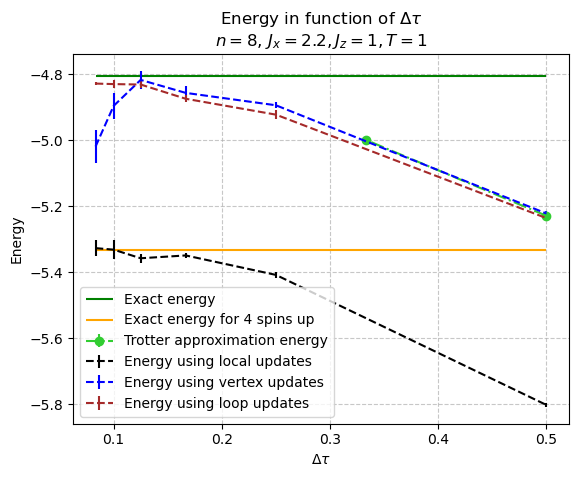
\includegraphics[width=\textwidth]{energy on dtau.png}
        \caption{Energy as a function of $\Delta\tau$}
        \label{fig:energy_tau_a}
    \end{subfigure}
    \hfill 
    \begin{subfigure}[]{0.48\textwidth}
        \centering
        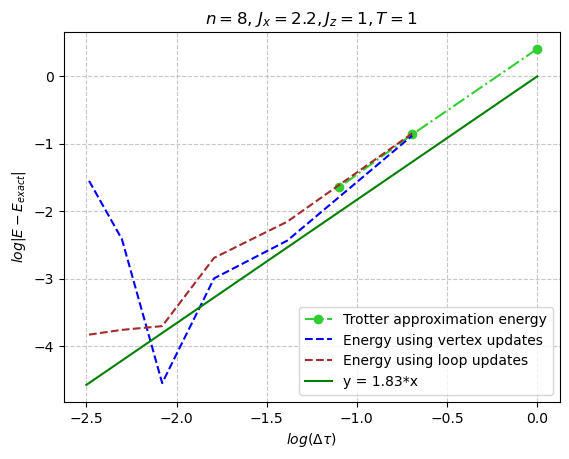
\includegraphics[width=\textwidth]{log(DE).png}
        \caption{Error in log scale}
        \label{fig:graphe_b2}
    \end{subfigure}
    \hfill
    \caption{Energy for 8 spin sites and different values of m plotted for different update methods}
    \label{fig:energy_tau}
\end{figure}

The energy error for all methods is dominated by the Trotter approximation at large $\Delta\tau$. However, for smaller values of $\Delta\tau$,the computed energies agree closely with the exact values, validating the model and suggesting the criterion $\Delta\tau \sim 0.1 J^{-1}$ for accurate calculations. \cref{fig:graphe_b2} indicates that the error scales as $\mathcal{O}(\Delta\tau^{1.83})$, which is consistent with the expected $\mathcal{O}(\Delta\tau^{2})$. The deviation observed for the vertex update is discussed in \cref{section_4_3}.

The advantage of the numerical methods becomes clear for larger systems, such as 10 spin sites and $m = 6$ as can be seen in \cref{fig:energy10*6}. The loop updates algorithm is able to calculate the energy for this larger system whereas the exact calculation was not possible.

\begin{figure}[!ht]
    \centering
        \includegraphics[width=0.6\textwidth]{energies_n.pdf}
        \caption{Energy as a function of the number of sites for m = 6}
    \label{fig:energy10*6}
\end{figure}
\newpage
\subsection{Spin correlation}

The model also allows computation of spin–spin correlation functions. Since each line represents a valid spin configuration, the correlation operator was averaged over all positions and imaginary-time slices:

\begin{equation}
    \left<S^z S^z_d\right> = \frac{1}{2mn} \sum_{j,i} S_{j,i}S_{j,i+d}
\end{equation}

The exact correlation is computed as in \cref{ss_d_exact} only on the first site (the value does not depend on the site).

\begin{equation} \label{ss_d_exact}
    \left<S^z S^z_d\right> = \frac{\text{Tr}\left(e^{-\beta H}S^z_0S^z_d\right)}{\text{Tr}\left(e^{-\beta H}\right)}
\end{equation}

The simulation accurately reproduced the correlations in both the ferromagnetic and antiferromagnetic regimes (\cref{spin_cor_n_8}).

\textit{Note: Other update schemes were not employed for this observable due to insufficient accuracy in their energy estimates.}

\begin{figure}
    \centering
    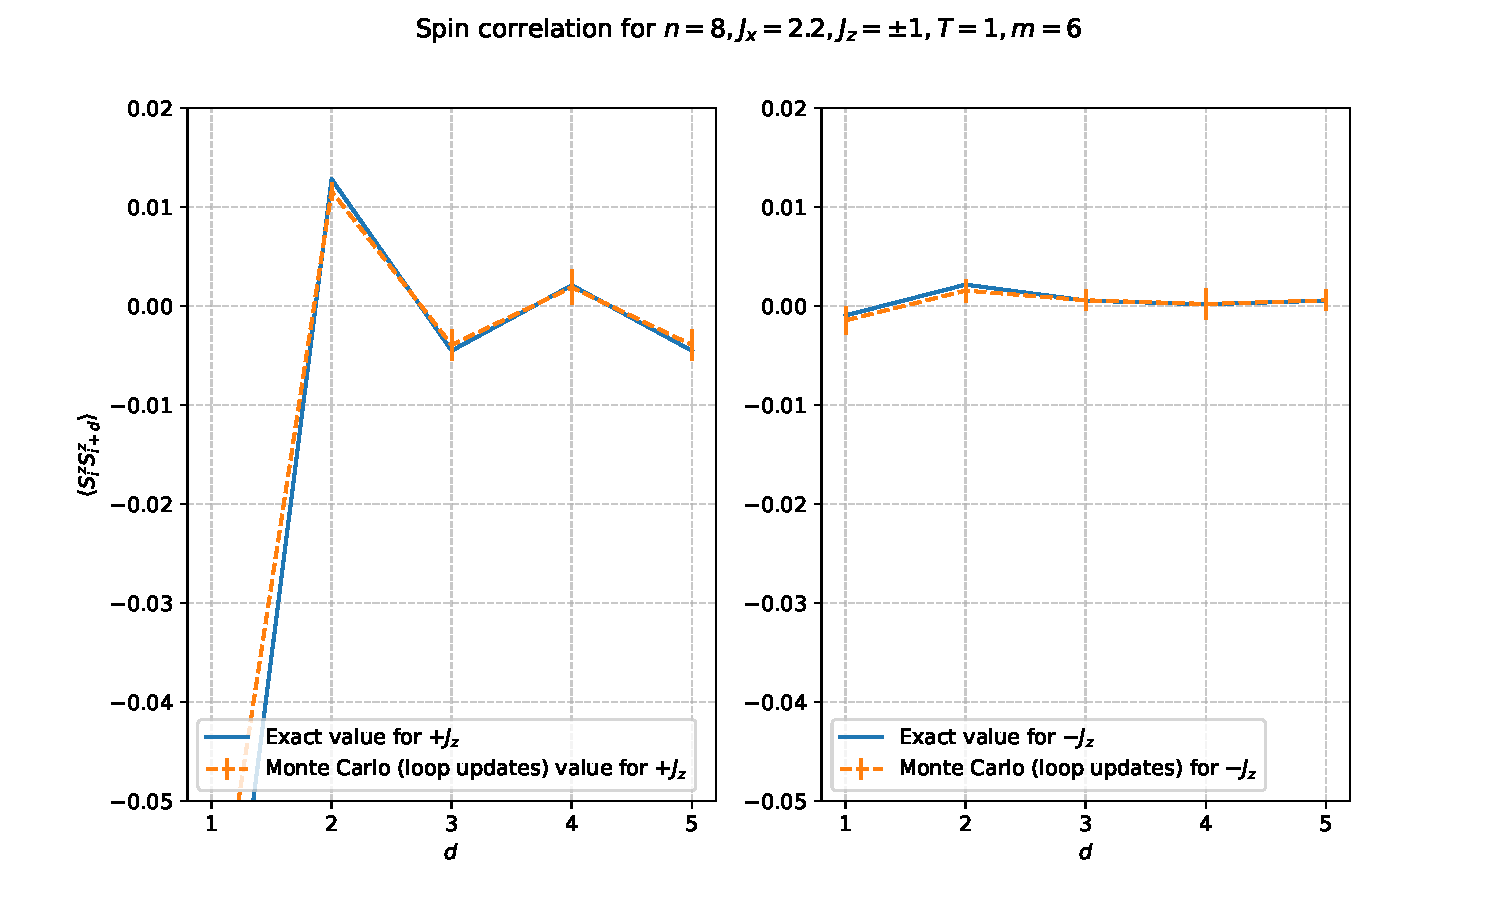
\includegraphics[width=\textwidth]{spin_correlation.pdf}
    \caption{Spin correlation computed using loop updates}
    \label{spin_cor_n_8}
\end{figure}

%We can also use our algorithm to see the impact of $J_x$ on the spin correlation. The results are presented in \cref{spins_j_x}. The results show that increasing $J_x$ strengthens spin correlations, as seen by the disappearance of the green regions.

The influence of the coupling $J_x$ on spin correlations was also examined (\cref{spins_j_x}). Increasing $J_x$ strengthens spin correlations, as reflected by the reduction of green regions in the heat map.

\begin{figure}
    \centering
    \includegraphics[width=\textwidth]{spins_J_x.pdf}
    \caption{Spin correlation as a function of $J_x$. \textit{The graphs must be understood as follows : the right heat-map shows mean correlations values on the $n_\text{rep}$ runs and the left heat-map gives the uncertainty ($\text{std}/\sqrt{n_\text{rep}}$) on each of the mean values of the right graph.}}
    \label{spins_j_x}
\end{figure}

\newpage
\subsection{Efficiency of the different update methods} \label{section_4_3}

The efficiency of each scheme was evaluated using two metrics: computation time (\cref{fig:comput_time}) and acceptance rate (\cref{table:3}).

\begin{figure}[!ht]
    \centering
    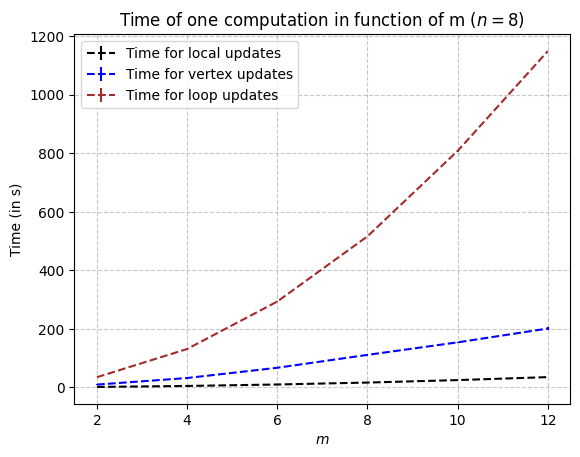
\includegraphics[width=0.8\textwidth]{cumputation time updates.png}
    \caption{Computation time for different update algorithms}
    \label{fig:comput_time}
\end{figure}

\begin{table}[!ht]
\centering
\begin{tabular}{|c | c | c | c | c| c | c |} 
 \hline
 m & 2 & 4 & 6 & 8 & 10 & 12 \\ [0.5ex] 
 \hline 
  Acceptance rate & 46,6 \% & 13,2 \% & 5,9 \% & 4,0 \%  & 3,3 \% & 2.5 \% \\ [0.5ex] 
 \hline
 

 
 
\end{tabular}
\caption{Acceptance rate for vertex update for $10^5$ tries}
\label{table:3}
\end{table}

Although the loop update requires longer computation times, its acceptance rate remains close to $100\%$, meaning that almost every proposed update results in a configuration change. However, for the vertex update the acceptance rate drops significantly as $m$ increases. Thus, for large $m$, roughly $50\times$ more trials are required to accept an update. This can be seen in \cref{fig:energy_tau}: for smaller $m$, the accuracy of the vertex update decreases. This is probably due to an insufficient amount of accepted updates leading to inaccurate calculations. To conclude, the high acceptance rate of the loop update is essential for obtaining accurate results on large systems, justifying its longer computation time. This qualitative analysis could be verified by calculating the autocorrelation time which measures the necessary number of steps to obtain a decorrelated configuration. Efficiency could be defined as the inverse of the product of the autocorrelation and computation times.
 
In summary, the loop update proved to be the most accurate and efficient method implemented.

\newpage

\printbibliography

\end{document}
